%% Section 3, Hands and who makes them. Converted from paper/sections/03_hands.md.
\section{Hands and who makes them}
\label{sec:hands}

\subsection{The design axes}
\label{sec:hands:axes}

% --- reproduced plates ------------------------------------------------------
% tex/figs/plates.tex defines one command per selected photograph. Load it here
% if nothing has loaded it already, so this section carries its own plates
% whether or not the preamble inputs the file. The \providecommand before each
% call makes a missing plate an empty command rather than an error. Every plate
% carries \pending: read tex/PERMISSIONS.md before this goes anywhere.
% ---------------------------------------------------------------------------
\makeatletter
\@ifundefined{plateLeapOverview}{\IfFileExists{figs/plates.tex}{% The one reproduced plate.
% Rebuilt from its source PDF by tools/relayout_plates.py; see tex/figs/SELECTED.md for the crop
% box and tex/PERMISSIONS.md for the licence it is used under.
%
% A plate is kept only where a photograph or a render carries something a drawing cannot, and
% only where the paper has the right to print it without asking anyone. Everything else that was
% reproduced has been redrawn in the paper's own style (figs/fig_transmission, fig_collision,
% fig_tactiledepth, fig_contactlabel, fig_retarget) or dropped, because the prose already made the
% point or because no honest drawing could be made from what the corpus records. That took
% eighteen plates to one, eleven visual styles to four, and eleven open permissions to none.
%
% The survivor is single column and single panel. It is not a `figure*`: a borrowed plate has not
% earned the page width.
%
% One command for it. A section author places it by writing
%   \plateGraspPenetration
% at the point in the section where the float should be anchored, once: a plate called twice
% prints twice, on two pages, under two numbers.
%
% The plate credits its source inside its own caption with \src or \cite, and carries \licensed as
% well, because its source is CC BY 4.0 and the licence asks for an attribution line.

% ========================================================== Sec. VI, two hands

\newcommand{\plateGraspPenetration}{%
  \begin{figure}[t]
    \centering
    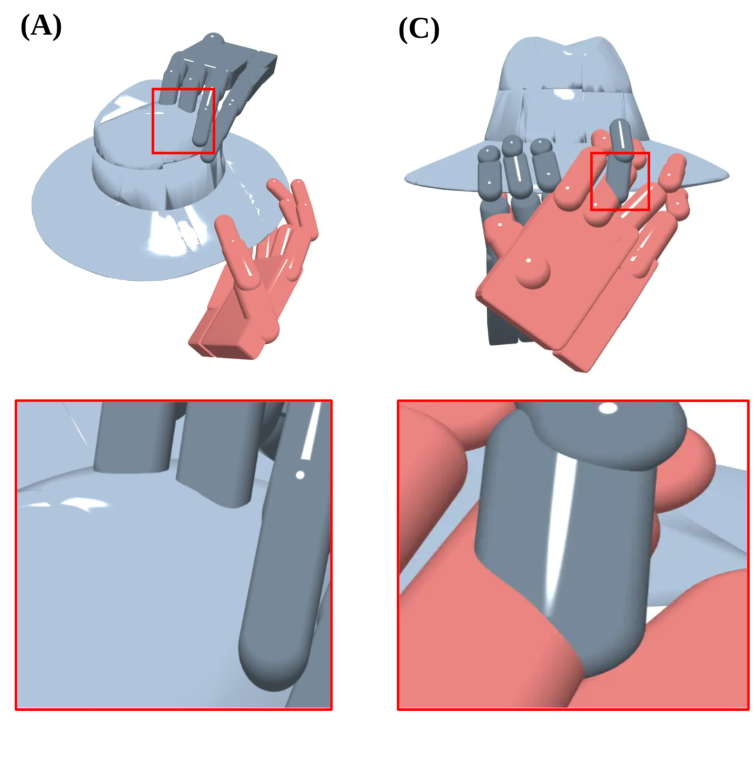
\includegraphics[width=0.86\columnwidth]{figs/selected/bimanual_grasp_penetration.png}
    \caption{Two failures of synthesised two-hand grasps, each enlarged at the
      contact: (A) a finger inside the object, (C) a finger inside the other hand.
      Both look plausible whole~\cite{bimangrasp_2024}.}
    \label{fig:bimanual-penetration}
    \licensed[panels (A) and (C) of Fig.~9]{Fig.~9 of Shao and Xiao, arXiv:2411.15903}{CC BY 4.0}{https://creativecommons.org/licenses/by/4.0/}
  \end{figure}}
}{}}{}
\makeatother

% A hand photograph at the head of the hardware section.
\providecommand{\plateLeapOverview}{}\plateLeapOverview


No degree-of-freedom, force, weight or price figure in Table~\ref{tab:hands-available} or
Table~\ref{tab:hands-announced}, both set in Appendix~\ref{app:tables}, was measured by anyone
outside the maker. Six rows are the exception, from peer-reviewed papers with stated protocols:
ILDA, Pisa/IIT, ORCA, RUKA, LEAP and BiDexHand. Every other claim is dated at its source.
Table~\ref{tab:hands-announced} prints the date beside each announced hand, and the dates for the
hands that can be bought are in the repository tabulation
(\texttt{paper/tables/table2\_hands\_available.md}, the \emph{claim date} column), which runs from
Shadow's specification of 4 December 2024 to vendor pages fetched on 17 September 2026.

The degree-of-freedom count is the first number a vendor states and the least comparable one.
Shadow's specification of 4 December 2024 reads ``20 actuated DOF and a further 4 under-actuated
movements for a total of 24 joints'' \cite{shadow_dexterous_hand_2005}. Table~\ref{tab:hands-available} prints joints first and
actuated DoF second, and the gap is the informative number. Where a vendor's own DoF figure
differs from the joint count, the joint count is what the table prints, as with Inspire's ``Degrees
of freedom 6, Numbers of joints 12'' \cite{inspire_rh56dfx_2023}. An actuator count is neither of those
two, and the repository tabulation keeps it in a column of its own. DexHand states no joint count at all, only 16 finger micro-servos and
two wrist servos, so 18 servos is the only count quotable for it \cite{dexhand_open_source_2023}. Daxo
states 120 actuators, no DoF figure, and a tendon structure with no rigid joints, which has far
fewer kinematic degrees of freedom than actuators \cite{daxo_muscle_v0_2025}.

% A transmission left exposed, beside the actuation-ratio argument.
\providecommand{\plateIldaLinkage}{}\plateIldaLinkage

The actuation ratio is the real decision. The Pisa/IIT SoftHand drives 19 joints from one motor and
its authors state the cost plainly: ``No in-hand dexterous manipulation is required for this
prototype'' \cite{pisa_iit_softhand_2014}. Tendon drive moves the motors off the fingers and the mass
follows them. Shadow's hand plus forearm weighs 4.3 kg, against 1.1 kg for the ILDA hand alone with
every motor in its palm \cite{shadow_dexterous_hand_2005,ilda_hand_2021}. ILDA states an 18 kg payload
against Shadow's 4 kg in a power grasp, and Shadow states no fingertip force at all. What tendons
cost is state estimation. The Faive Hand estimated joint angles from tendon length through a Kalman
filter and its cube reorientation failed on hardware, which its authors blamed on ``poor joint angle
measurement from the EKFs, especially when there is contact'' \cite{faive_hand_2023}. Ruka-v2 adds
detachable AS5600 encoders to measure that problem rather than close the loop on it, and those
encoders put its open-loop linear joint-to-motor map at 8.26 degrees of error over seven joints
\cite{ruka_v2_2026}.

% The linkage that cuts the actuator count, beside the coupling argument.
\providecommand{\plateCoupledLinkage}{}\plateCoupledLinkage

Direct drive trades torque density for transparency. LEAP's Dynamixel joints resist 19.5 N in a
pull-out test against the Allegro Hand's 8.5 N, at 595 g for the LEAP hand \cite{leap_hand_2023}, and
the Allegro's own weight has no reachable source. Linkage drive is the argument against the
forearm. ILDA puts 15 motors, drivers and ball screws inside the palm and reports 34 N at the
fingertip in the bent pose and 28 N stretched \cite{ilda_hand_2021}. Linkages buy coupling for free, as
in BiDexHand's four-bar that drives each DIP off its PIP, whose paper claims 16 actuated DoF and 21
joints while its README describes 15 servos driving 15 joints \cite{bidexhand_2025}.

Fingertip force is the number a hand buyer reads first, and across these rows it is six different
measurements. Table~\ref{tab:hands-available} puts the quantity beside the figure: pull-out resistance for
LEAP's 19.5 N, pinch for RUKA's 2.74 N and BrainCo's 15 N, fingertip normal force under a 1 cm
indenter for Unitree's 10 N, a calibrated five-trial fingertip force for BiDexHand's 2.14 N, a
peak vendor claim for 1X's 45 N, and two unlabelled spec columns for Sharpa's ``20 N \textbar{} 12 N''.
BrainCo's whole-fist grip of 50 N is a separate figure and is no longer in the same column as a
pinch. ORCA's 19.6 N was none of these. It is the newton equivalent of a 2 kg index-finger payload
at a fixed 600 mA motor current, so its force cell is empty and the figure is recorded as a payload
instead \cite{orca_hand_2025}. Payload is no more comparable than force, which is why
Table~\ref{tab:hands-available} does not print it. Nine of its twenty hands state one, in the
repository tabulation (\texttt{paper/tables/table2\_hands\_available.md}, the \emph{payload}
column), and no two state it under the same test: Shadow 4 kg in a power grasp with no protocol
given, Tesollo 2.5 kg pinching and 10 kg enveloping as rated figures, Unitree 3.5 kg palm-down and
4.5 kg palm-left on a 5 cm round object, ORCA 10.5 kg on four fingers and 2 kg on the index alone at
a fixed motor current, BiDexHand 4.54 kg lifted, and RUKA 6.0 kg as the weight at which its
joint-angle error passes 15 degrees.

Compliance is repairability seen twice over, and both are mechanical fuses: the Pisa/IIT
SoftHand's rolling-contact joints return to assembly after over-extension and ORCA's ``poppable''
pin joints dislocate rather than break \cite{pisa_iit_softhand_2014,orca_hand_2025}. ORCA also reports
tendon drive as maintenance: ``Prolonged use requires manual re-tensioning to maintain performance''.
What fails is rarely the motors. Its durability run found silicone skin degrading on two fingertips
after about 2,000 to 4,000 grasp cycles and sensor wires snapping on three after about 4,500 to
7,000. The sensing wore out an order of magnitude sooner than the hand.

Two properties matter before any of the above, and neither is a column of
Table~\ref{tab:hands-available}: both are in the repository tabulation, which prints a
\emph{control rate} and a \emph{URDF or MJCF} column for every row
(\texttt{paper/tables/table2\_hands\_available.md}). The first is the rate a loop can be
closed at, which spans 250 Hz on a Tesollo to 1 kHz on a Shadow, a Unitree or a Wuji, with the
Allegro at 333 Hz on its own CAN clock and Inspire stating no rate at all. LEAP's 500 Hz is a
serial query ceiling and its own sim-to-real policy runs at 20 Hz, which answer different questions
\cite{leap_hand_2023}. A reader deploying torque control is bitten by that first. The second is
whether a URDF or MJCF exists and who ships it, which is the bridge to Section~\ref{sec:simulators} and to this
survey's recommendation to pick a hand a simulator already carries. Shadow, Sharpa, Wuji, the
Ability Hand, RUKA, Faive and the Allegro driver ship one. LEAP is the warning: its paper says the
URDF is released and the released API repository contains none \cite{leap_hand_2023}.

% ---------------------------------------------------------------------------
% Table 2, the hands that can be bought or built, is set in Appendix B rather than here. It is
% consulted rather than read, so it is reference material; see the head of Appendix B.
% ---------------------------------------------------------------------------

\subsection{The hands the research literature actually runs on}
\label{sec:hands:used}

% ---------------------------------------------------------------------------
% Figure 2. The bar chart is wider than a column at its natural size, so it is
% scaled to the column rather than left to overflow.
% ---------------------------------------------------------------------------
\begin{figure}[!t]
  \centering
  \resizebox{\columnwidth}{!}{% generated by tools/make_tikz_figures.py; do not edit
\begin{tikzpicture}[
  font=\footnotesize,
  bar/.style={draw=none,fill=black!62},
  barlight/.style={draw=none,fill=black!22},
  baracc/.style={draw=none,fill=accent},
  box/.style={draw=black!45,line width=0.3pt,inner sep=3pt,align=left},
  ghost/.style={draw=black!35,line width=0.3pt,dash pattern=on 1.4pt off 1.4pt,inner sep=3pt,align=left},
  lnk/.style={draw=black!38,line width=0.28pt},
  lbl/.style={font=\scriptsize},
  num/.style={font=\scriptsize\color{black!55}},
]

\node[lbl,anchor=east] at (0,-0.00) {Allegro};
\fill[bar] (0.12,-0.09) rectangle (6.52,0.09);
\node[num,anchor=west] at (6.62,-0.00) {35};
\node[lbl,anchor=east] at (0,-0.36) {Shadow or Adroit};
\fill[bar] (0.12,-0.45) rectangle (4.51,-0.27);
\node[num,anchor=west] at (4.61,-0.36) {24};
\node[lbl,anchor=east] at (0,-0.72) {Inspire};
\fill[bar] (0.12,-0.80) rectangle (3.59,-0.64);
\node[num,anchor=west] at (3.69,-0.72) {19};
\node[lbl,anchor=east] at (0,-1.08) {LEAP};
\fill[bar] (0.12,-1.17) rectangle (2.31,-1.00);
\node[num,anchor=west] at (2.41,-1.08) {12};
\node[lbl,anchor=east] at (0,-1.44) {parallel-jaw gripper};
\fill[baracc] (0.12,-1.52) rectangle (2.31,-1.35);
\node[num,anchor=west] at (2.41,-1.44) {12};
\node[lbl,anchor=east] at (0,-1.80) {XHand};
\fill[bar] (0.12,-1.88) rectangle (1.58,-1.71);
\node[num,anchor=west] at (1.68,-1.80) {8};
\node[lbl,anchor=east] at (0,-2.16) {Ability};
\fill[bar] (0.12,-2.24) rectangle (1.40,-2.07);
\node[num,anchor=west] at (1.50,-2.16) {7};
\node[lbl,anchor=east] at (0,-2.52) {Sharpa};
\fill[bar] (0.12,-2.60) rectangle (1.22,-2.43);
\node[num,anchor=west] at (1.32,-2.52) {6};
\node[lbl,anchor=east] at (0,-2.88) {Fourier};
\fill[bar] (0.12,-2.96) rectangle (0.67,-2.79);
\node[num,anchor=west] at (0.77,-2.88) {3};
\node[lbl,anchor=east] at (0,-3.24) {D'Claw or TriFinger};
\fill[bar] (0.12,-3.32) rectangle (0.49,-3.15);
\node[num,anchor=west] at (0.59,-3.24) {2};
\node[lbl,anchor=east] at (0,-3.60) {Wuji};
\fill[bar] (0.12,-3.68) rectangle (0.49,-3.51);
\node[num,anchor=west] at (0.59,-3.60) {2};
\node[lbl,anchor=east] at (0,-3.96) {Faive};
\fill[bar] (0.12,-4.04) rectangle (0.30,-3.87);
\node[num,anchor=west] at (0.40,-3.96) {1};
\end{tikzpicture}}
  \caption{Which hands the literature actually runs on. Per hand, the number of method papers
  whose own experiments use it. Of 112 method rows, 103 name a hand, and a paper
  using two hands is counted under both. The accented bar is the parallel-jaw gripper, which is
  not a dexterous hand, and only three dexterous hands carry more method rows than it. The Adroit
  is the MuJoCo model of a Shadow hand and takes a line of its own, three of whose four rows name
  no Shadow, so the Shadow bar is the rows that name a Shadow itself. Only
  hands with at least one method row appear, so the nine company-announced hands of
  Table~\ref{tab:hands-announced} and the hands of Table~\ref{tab:hands-available}
  that no paper runs on are absent from the chart.}
  \label{fig:hands}
\end{figure}

% Research hands photographed to scale, beside the count of who runs on what.
\providecommand{\plateHandScale}{}\plateHandScale

The two oldest designs in Table~\ref{tab:hands-available} carry 49 of the 103 method rows that name a hand at all, and
seven rows use both. Neither design's date is confirmed by its own sources, so 2005 and 2016 are
the bibliography's. \figurename~\ref{fig:hands} counts, per hand, the method papers whose own experiments use it. Of
112 method rows, 103 name a hand. The Allegro accounts for 35, Shadow for 21, the Inspire RH56
family for 19, a parallel-jaw gripper for 12 and LEAP for 12. Seventy-five of the 103 name an
Allegro, a Shadow or Adroit model, LEAP or an Inspire.

The Allegro's position is the uncomfortable part. Its product page at allegrohand.com/v4 returned
HTTP 404 while the Wonik wiki timed out \cite{allegro_hand_v4_2016}. Everything Table~\ref{tab:hands-available} confirms about
the most-used hand in the corpus comes from its ROS driver: 16 joints, four fingers, a torque
interface, a 333 Hz CAN clock, 12 V, no tactile sensing. Its weight, joint torque, payload and
price have no reachable source. The field's most common platform cannot be specified from a page a
reader can open.

Concentration would matter less if the hand did not move the result, and it does. On the same
simulated cube rotation, LEAP reaches 0.2288 rad/s against the Allegro's 0.0828 rad/s
\cite{leap_hand_2023}, and RUKA reports a 2.74 N pinch against the Allegro's 1.60 N under the same
three-trial pinch test \cite{ruka_2025}. A method compared only on Allegro hardware is compared at one
point in a space where a single axis moves the headline number two or three times over. Two further
patterns follow. Inspire, XHand and Sharpa take 29 of the 103 rows between them, four rows use two
of the three, and none is earlier than 2024. Eight take none at all: ORCA, RUKA, Ruka-v2,
BiDexHand, DexHand, the Proception ProHand, the Tesollo DG-5F and the Unitree Dex5.

\subsection{Open hardware and the collapse in cost}
\label{sec:hands:open}

Six rows in Table~\ref{tab:hands-available} are open hardware, and LEAP Hand V2 in
Table~\ref{tab:hands-announced} is a seventh. Five of the seven state a dollar cost: \$2,000 for
LEAP, \$3,000 for LEAP Hand V2, \$1,500 for Ruka-v2, \$1,300 for RUKA and \$300 for DexHand. ORCA
states a material cost below 2,000 CHF that the price column leaves unconverted, and BiDexHand
states none \cite{orca_hand_2025,bidexhand_2025}. The Faive Hand states neither a cost nor a licence that could be
read, so it is not counted as open hardware here \cite{faive_hand_2023}. Two of the stated bases need
saying. DexHand's \$300 is ``additional total cost of components'', excluding the printing and the
wrist servos \cite{dexhand_open_source_2023}, and ORCA's own figure sits against Ruka-v2's table listing
ORCA at about \$3.5K \cite{ruka_v2_2026}.

The expensive end of the collapse is secondhand throughout. The only six-figure numbers on disk are
RUKA's comparison table at \$100,000 for a Shadow Hand and Faive's ``steep price tag of 110k GBP''
\cite{ruka_2025,faive_hand_2023}. Shadow's own page says to discuss pricing and Table~\ref{tab:hands-available}'s price cell
for it is empty. The collapse is real at the cheap end and secondhand at the expensive one, and it
has barely moved the literature. Twelve of the 103 hand-naming method rows use an open-hardware
hand, and all twelve are LEAP.

What the cheap hands give up is sensing. LEAP has none and names touch sensors as future work
\cite{leap_hand_2023}, RUKA states its design ``lacks tactile sensing'' \cite{ruka_2025}, and BiDexHand's
sources never mention touch \cite{bidexhand_2025}. ORCA is the exception, with binary FSR fingertips
whose threshold was measured as low as 0.05 N on a fresh fingertip, against the sensor's rated
0.29 N, and 6.38 N on a degraded one \cite{orca_hand_2025}.

\subsection{Announced and unreleased hands}
\label{sec:hands:announced}

Behind Table~\ref{tab:hands-announced}'s rows sit three kinds of evidence, and conflating them is how a DoF figure with no
source ends up in a survey. Vendor prose carrying numbers is the strongest, as on 1X's page of
9 July 2026 \cite{onex_neo_hand_2026}. Video is second and carries none. Press or bibliography assertion
is third, as with Tesla's V3 hand, known here only through a paraphrase of patents because the
USPTO PDF parsed empty \cite{tesla_optimus_hand_2025}. Table~\ref{tab:hands-announced} blanks the cells resting on the third
class and footnotes who did the arithmetic.

A survey can go one step past recording that a claim is unverified, which is to say which claims
are implausible on their face. Daxo's 120 actuators in 750 g is about 6 g per actuator including
structure, tendons, routing and skin \cite{daxo_muscle_v0_2025}. Clone's 27 degrees of freedom under
2 pounds excludes a 500 W pump the source does not confirm is excluded \cite{clone_robotics_hand_2024}.
Figure 03's ``Degrees of freedom, hands \textbar{} 20'' sits on the same tracker page as ``Number of fingers \textbar{}
10'', so it is almost certainly the pair \cite{figure_03_hand_2025}. Tesla's repeated 22 is one article's
arithmetic of four DoF on each of five fingers plus two at the wrist, and Gen 2's own figure was 11
\cite{tesla_optimus_hand_2025}.

Scepticism belongs to the evidence class, not to which table a row lands in. Sharpa's 22 of 22,
Wuji's 20 of 20 and Tesollo's 20 of 20 are vendor claims about unmeasured hardware and they sit in
Table~\ref{tab:hands-available}, where Sharpa's page footnotes ``Specifications may vary between products'' and Wuji's says
the spec ``will continue to iterate'' on a Beta1 product \cite{sharpa_wave_2026,wuji_hand_2025}. Even
the best-specified vendor page in the corpus leaves its fingertip-force columns unlabelled.

% ---------------------------------------------------------------------------
% Table 3, the announced and unreleased hands, is set in Appendix B rather than here.
% ---------------------------------------------------------------------------

\subsection{Tactile sensing as part of the hand}
\label{sec:hands:tactile}

% Vision-based tactile sensors used as the fingertips themselves.
\providecommand{\plateDigitFingertips}{}\plateDigitFingertips

DIGIT set the cost floor. It is 20 by 27 by 18 mm, weighs about 20 g, streams 640x480 at 60 fps,
and its paper states a ``total estimated manufacturing cost is approximately 15 USD per sensor ...
when manufactured in a batch of 1000'' \cite{digit_2020}. Durability was as much the contribution as
price: its gel degraded 0.3 percent over 15 abrasion passes, against 805 and 918 percent for the
two gels compared with it.

Digit 360 is the same lineage at a different operating point, claiming about 8.3 million taxels,
spatial features to 7 um, normal and shear force resolution of 1.01 mN and 1.27 mN, and on-device
processing that cuts event-to-action latency from 6 ms to 1.2 ms \cite{digit360_2024}. It is also not
for sale, and no corpus paper's parsed text names it.

% A pad fitted to a commercial hand: the other way to change what a fingertip does.
\providecommand{\plateInspireTactilePad}{}\plateInspireTactilePad

XELA's uSkin is the non-camera alternative and the one that bolts onto hands the field already
uses. Its curved fingertip kit for the Allegro V4 and LEAP carries 30 three-axis sensing points, a
full Allegro integration reaches 368, resolution is 0.1 gram-force, and the kit runs at 275 Hz
\cite{xela_uskin_2020}. The 500 Hz figure often quoted belongs to the product family, not the curved
fingertip. One corpus paper names it, \cite{sparsh_2024}, whose self-supervised encoders are pre-trained
on 462.7k tactile images and beat matched end-to-end models by 95.1 percent when both see 33 to 50
percent of the labels. Its own bead-maze policies never complete the maze on the real robot.

The usage number is the one to keep, and it needs its inclusion rule stated: a sensor physically on
the hand, read by the deployed policy. Eight of 112 method rows meet it: \cite{anyrotate_2024,articulated_tools_inhand_2025,dexteleop0_2026,dexumi_2025,hato_visuotactile_2024,robot_synesthesia_2023,rotateit_2023} and \cite{rotating_without_seeing_2023}. The rule excludes
\cite{penspin_2024}, whose 20 binary contacts are simulated on an Allegro that has no tactile hardware
and whose released config sets \texttt{enable\_tactile: False}, and it excludes \cite{dexndm_2025} and
\cite{dexplore_2025} for the same reason. Sixty-five of the 112 method papers mention tactile sensing
somewhere, which is the gap worth quoting. Thirty-five is the count over this survey's notes.

Almost none of the eight uses a high-resolution sensor. Yin et al.
\cite{rotating_without_seeing_2023} remove vision entirely and rotate objects from 16 binary touch
sensors over the palm, links and fingertips, deployed zero-shot to a real Allegro, and Robot
Synesthesia uses 16 force-sensing resistors read as binary \cite{robot_synesthesia_2023}. Two papers
exclude touch deliberately, HORA reporting rotation ``even without the usage of vision and tactile
sensing'' \cite{hora_2022}, and ORCA's authors dropping it from their reinforcement learning ``due
to the additional complexity involved in accurately modeling them'' \cite{orca_hand_2025}. Taxel
counts have risen by three orders of magnitude while the policies consuming them have stayed at
binary contact.

\subsection{What is sold against what is published on}
\label{sec:hands:gap}

The hands missing from \figurename~\ref{fig:hands} carry the finding. None of the nine company-announced hands in Table~\ref{tab:hands-announced}
appears in a single method row whose own experiments use it. Tesla, Figure, 1X, Sanctuary, Boston
Dynamics, Xiaomi, Clone, Daxo and PaXini account for zero of the 112 method papers' experiments.
The nearest thing to a counterexample is \cite{helix_2025}, a Figure blog post claiming a 35-DoF
whole-upper-body action space at 200 Hz that includes individual finger control. It never names the
hand, gives no per-hand DoF count, and reports no success rate or trial count for any task. It is
the maker describing its own unreleased hand, which is the evidence class the finding is about. The
four research prototypes in Table~\ref{tab:hands-announced} are in a different position, since the Faive Hand and LEAP Hand
v2 Advanced account for three method rows between them \cite{graspxl_2024,bidex_teleop_2024}.

Table~\ref{tab:hands-announced}'s emptiness is measurable and part of the same finding. Over the
eight specification columns it prints, from DoF to price, 58 percent of its cells are values no
source stated, against 42 percent for the hands that can be bought; both captions state their own
count. Over the twelve specification columns the repository tabulation carries, the same split is 61
to 39. The hands with the highest advertised DoF counts have the least specification behind
them.

The one hand that crosses the gap crosses it because its maker published rather than announced.
ByteDexter reaches a method row through a ByteDance technical report stating 21 DoF per hand, 16
piezoresistive fingertip channels in the action vector and real-robot success rates
\cite{gr_dexter_2025}, not through a product page. That mechanism is available to every vendor in
Table~\ref{tab:hands-announced} and none has used it.

The gap runs the other way too, and the last column of Table~\ref{tab:hands-available} shows it. Eight hands that can be bought
or built from published designs take zero method rows each: the Unitree Dex5 with 94 pressure
sensors on its P variant \cite{unitree_dex5_2025}, the fully actuated Tesollo DG-5F
\cite{tesollo_dg5f_2024}, the 22-DoF Proception ProHand \cite{proception_prohand_2026}, ORCA, RUKA,
Ruka-v2, BiDexHand and DexHand. Cheapness is established only for RUKA, Ruka-v2 and DexHand,
because Table~\ref{tab:hands-available}'s price cell is empty for Unitree, Tesollo, the ProHand,
ORCA and BiDexHand, and the only Dex5
price on disk is Ruka-v2's secondhand ``\textasciitilde{}\$25K'' \cite{ruka_v2_2026}. A reader choosing a hand on this
corpus's evidence has two well-precedented options, an Allegro or an Inspire, and a third in LEAP
if twelve papers is enough. Everything else is a press release or a hand nobody has published on.
